\section{Мета роботи}
Набути досвіду практичної роботи з бінарними деревами.

\noindent
\textbf{Теми для попередньої роботи:}
\begin{itemize}
    \item нелінійні списки;
    \item графи;
    \item дерева;
    \item операції на деревах.
\end{itemize}


\section{Завдання}
Розробити програму, що дозволяє створити бінарне дерево та
вирішити індивідуальне завдання. У завданнях 7 – 16 включно (де не вказані
обходи) реалізувати два алгоритми обходу, які обрати самостійно.

Розробити програму турнірного сортування.


\section{Хід виконання}
Для виконання завдання було обрано мову Rust.
Увесь код також додатково був розміщений в GitHub репозитарії: \href{https://github.com/blackgolyb/algos-labs}{https://github.com/blackgolyb/algos-labs}.


\newpage
\subsection{Турнірне сортування}
\lstinputlisting[language=Rust, style=colouredRust]{\codeDirectory/src/libs/sort/variants/tournament.rs}


\newpage
\subsection{Приклад роботи програми}
\noindent
Код програми для перевірки:
\lstinputlisting[language=Rust, style=colouredRust]{\codeDirectory/src/labs/lab13/main.rs}


\begin{figure}[ht!]
    \centering
    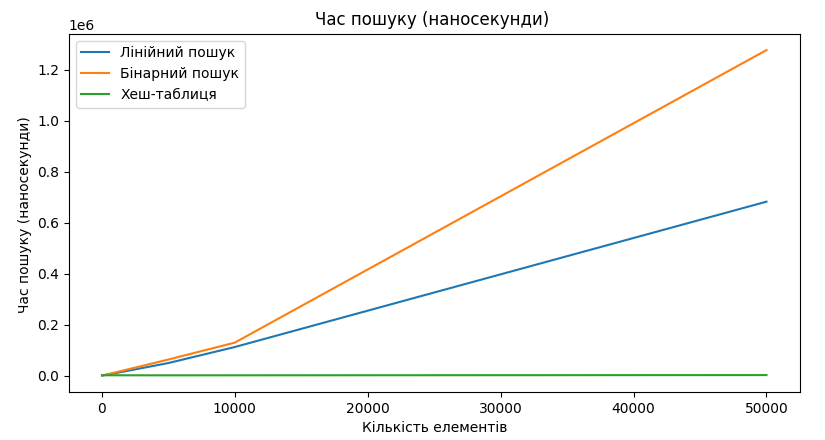
\includegraphics[width=.8\textwidth]{\assetsDirectory/time.png}
    \caption{Залежність часу пошуку від кількості елементів}
\end{figure}
\begin{figure}[ht!]
    \centering
    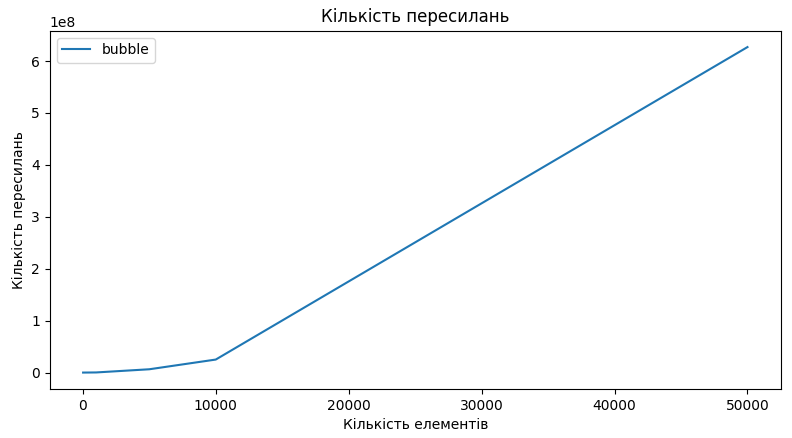
\includegraphics[width=.8\textwidth]{\assetsDirectory/swap.png}
    \caption{Залежність кількості пересилань від кількості елементів}
\end{figure}
\begin{figure}[ht!]
    \centering
    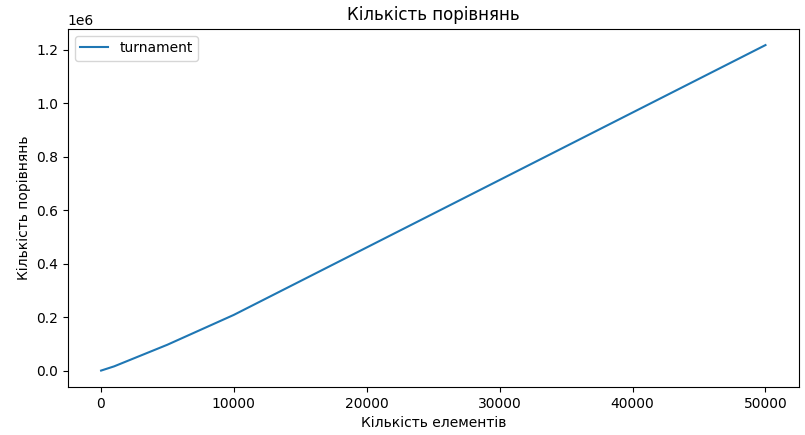
\includegraphics[width=.8\textwidth]{\assetsDirectory/comp.png}
    \caption{Залежність кількості порівнянь від кількості елементів}
\end{figure}


\newpage
\section{Висновки}
В ході виконання лабораторної робити було створено турнірне сортуванн.
Також його було протестовано на різних обємах даних та побудовано графіки для наглядної демонстрації характеристик характеристик.
